% -*- root: dissertation.tex -*-
\section{Findings}

\subsection{QP$_1$ Code smells specific to the Android Presentation Layer}
\label{phase1-results}

In this section we present general results on the process of deriving code smells (Section \ref{phase1-general-results}) and the catalog with 20 proposed code smells related to the Android presentation layer (Section \ref{phase1-code-smells-derivation}).

\subsubsection{General Results and Findings}
\label{phase1-general-results}

All 16 questions about good and bad practices in the elements of the Android presentation layer (second section of S$_1$) were optional, so some received more answers than others. The figure \ref{fig:ElementsVSAnswers} displays the total answers received for each question. We can observe that 35 of the 45 respondents answered the question about good practices in \textit{Activities}: ``\textit{Do you have any good practices to deal with Activities?}''. While 38 responded answered the question about bad practices in \textit{Activities}: ``\textit{Do you have anything you consider bad practice when dealing with Activities?}''.

\begin{figure*}[!htb]
\centering
% \hspace*{-0.7cm}
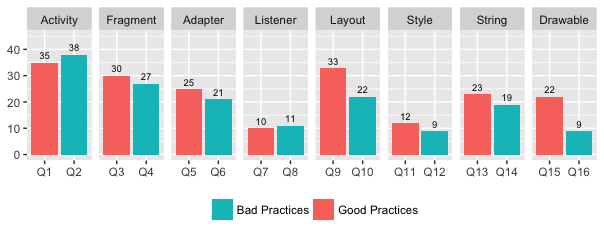
\includegraphics[width=.8\linewidth]{phase1-survey-answers3-en.png}
\caption{Total answers for each question about good and bad practices in the eight elements of the Android presentation layer.}
\label{fig:ElementsVSAnswers}
\end{figure*}

The element that received the least answers about \textbf{\small good practices} was \textit{Listener}, being answered by 10 of the 45 participants. The elements that received the least responses over \textbf{\small bad practices} were the \textit{Style} resources and \textit{Drawable}, both of which were answered by only 9 of the 45 participants. Among the components, the ones that received the most responses were \textit{Activities} and \textit{Fragments}, both being answered by at least 27 participants. Among the resources, the one that received the most response was the \textit{Layout} resource, being answered by at least 22 of the 45 participants. Overall, good practice questions were answered more than the bad practice questions, except for \textit{Activities} and \textit{Listeners}.

The coding process resulted in 46 categories, from which we considered for the derivation of bad smells all those that presented occurrences greater than or equal to five, based on the number of Nielsen \cite{NielsenMagicNumber:00}. Thus, 22 categories were considered. Of these 22, we disregarded 2 more because they were (i) a traditional bad smell (Large Class) and (ii) one aspect of object orientation (Inheritance). Resulting in 20 categories for deriving the bad smells of the Android presentation layer.

The Table \ref{tab:CategoriesVSFrequency} displays the total number of occurrences segmented by element of the Android presentation layer of the 20 categories considered for the derivation of bad smells. For example, the category \textsc{\small Brain UI Component} displays 29 in the \textit{Activity} column, 16 in the \textit{Fragment} column, 14 in the \textit{Adapter} column, and 1 in the \textit{Listener}, this means that 29 occurrences were in responses on good and bad practices in \textit{Activities}, 16 occurrences were in responses on good and bad practices in \textit{Fragments}, and so on. The superscript number, in parentheses, next to the category name indicates the total number of occurrences, that is, the sum of occurrences on all Android elements.


In Figure \ref{fig:ElementsVSAnswers} the total responses on good and bad practices in Activities is 73 (summation of columns Q1 and Q2), and in Table \ref{tab:CategoriesVSFrequency} the total responses in the Activity column is 49. This difference occurs because in the figure we are considering the answers of all 46 categories, while in the table we consider only the answers to the 20 categories considered.

\begin{table*}[!htb]
\centering
\renewcommand*{\arraystretch}{1}
\caption{Total responses on good and bad practices in each element of the Android presentation layer.}
\footnotesize
\begin{tabular}{@{}p{7cm}@{}cccccccccp{3cm}}
\toprule
\textbf{Mau Cheiro} & \rot[32][2em]{\textbf{Activity}} & \rot[32][2em]{\textbf{Fragment}} & \rot[32][2em]{\textbf{Adapter}} & \rot[32][2em]{\textbf{Listener}} & \rot[32][2em]{\textbf{Layout}} & \rot[32][2em]{\textbf{String}} & \rot[32][2em]{\textbf{Style}} & \rot[32][2em]{\textbf{Drawable}} \\
\toprule
\textsc{Brain UI Component}$^{(60)}$       & 29  & 16  & 14  & 1   & -    & -   & -   & -  &  \\
\textsc{Coupled UI Component}$^{(18)}$      & 2   & 10  & 3   & 3   & -    & -   & -   & -  &  \\
\textsc{Suspicious Behavior}$^{(17)}$         & 4   & -   & 3   & 10  & -    & -   & -   & -  &  \\
\textsc{Fool Adapter}$^{(13)}$             & -   & -   & 13  & -   & -    & -   & -   & -  &  \\
\textsc{Excessive Use Of Fragments}$^{(9)}$      & -   & 9   & -   & -   & -    & -   & -   & -  &  \\
\textsc{UI Component Doing IO}$^{(9)}$     & 5   & 3   & 1   & -   & -    & -   & -   & -  &  \\
\textsc{No Fragment Usage}$^{(8)}$             & 4   & 4   & -   & -   & -    & -   & -   & -  &  \\
\textsc{Absence of Architecture}$^{(6)}$         & 4   & 2   & -   & -   & -    & -   & -   & -  &  \\
\textsc{Flex Adapter}$^{(6)}$                & -   & -   & 5   & -   & 1    & -   & -   & -  &  \\
\textsc{Resource Name Non Patterned}$^{(24)}$ & -   & -   & -   & -   & 5    & 10  & 5   & 3  &  \\
\textsc{Magic Resource}$^{(23)}$                 & -   & -   & -   & -   & 6    & 15  & 2   & -  &  \\
\textsc{Deep Nested Layout}$^{(19)}$  & -   & -   & 1   & -   & 18   & -   & -   & -  &  \\
\textsc{Avoid Tradicional Images}$^{(18)}$ & -   & -   & -   & -   & 1    & -   & -   & 17 &  \\
\textsc{Layout Long or Repeated}$^{(14)}$       & -   & -   & -   & -   & 14   & -   & -   & -  &  \\
\textsc{Missing Image}$^{(12)}$                & -   & -   & -   & -   & 2    & -   & -   & 10 &  \\
\textsc{God Style Resource}$^{(8)}$         & -   & -   & -   & -   & -    & -   & 8   & -  &  \\
\textsc{Messy String Resource}$^{(8)}$     & -   & -   & -   & -   & -    & 8   & -   & -  &  \\
\textsc{Repeated Style Attributes}$^{(7)}$   & -   & -   & -   & -   & 3    & -   & 4   & -  &  \\
\textsc{Inappropriate String Reuse}$^{(6)}$      & -   & -   & -   & -   & -    & 6   & -   & -  &  \\
\textsc{Hided Listener}$^{(5)}$              & -   & -   & -   & 5   & -    & -   & -   & -  &  \\
\bottomrule
\end{tabular}
\label{tab:CategoriesVSFrequency}
\end{table*}

It is worth noting that the same code smell can affect more than one element of the Android presentation layer. By means of the table \ref{tab:CategoriesVSFrequency}, we can get suggestions on what Android elements a code smell affects by crossing the number of occurrences, that is, if there are occurrences, possibly the respective code smell affects the respective element. For example, the code smell \textsc{\small UI Brain Component} is presented in 4 components: \textit{Activities} with 29 occurrences, \textit{Fragments} with 16, \textit{Adapters} with 14 and \textit{Listeners} with 1, and in fact, that code smell can affect all those components.

However, for other code smells, this suggestion is not true. For example, in the case of the code smell \textsc{\small Deep Nested Layout}, although there is 1 occurrence in \textit{Adapter}, that code smell does not affect it. The response that gave rise to this occurrence actually indicated good practice in layouts: \textit{``Create really light layouts.''}~(P36). This type of analysis of the response was carefully performed for writing the textual definition of code smells to be presented in the next section.


\subsubsection{Proposed Code Smells}
\label{phase1-code-smells-derivation}

Table \ref{tab:Smells} presents the list and a brief description of the 20 proposed Android code smells derived from the 20 categories with five occurrences or more, resulting from the coding process. The first 9 code smells affect Android presentation layer components, the next 11 affect Android resources.

Definitions were based on the answers obtained \footnote{All English text has been translated freely throughout the dissertation}. For example, some responses that supported the code smell \textsc{\small UI Brain Component} were: \textit{``Do Business Logic [in Activities]''} (P16). ``\textit{Putting business rule on Adapter}'' (P19), \textit{``Keep business logic in Fragments''} (P11), \textit{``Activities represent a single screen and only interact with the UI, any logic must be delegated to another class''} (P16) where P1 to P45 represent each of the respondents. In order to make the reading simpler, the answers used to base them are available in Appendix \ref{appendix:smells-purpose-of-solution}.

In the following paragraphs we present in a textual way the definition of code smells, as well as the elements affected by each code smell and related symptoms.

\begin{table*}[htb!]
\centering
\renewcommand*{\arraystretch}{1}
\caption{List of 20 code smells in the Android presentation layer and brief description of the symptoms.}
\footnotesize
\begin{tabular}{@{}p{6.6cm}@{}p{10cm}@{}}
\toprule
\textbf{Nome} & \textbf{Descrição} \\
\toprule
\textsc{Brain UI Component}$^{(60)}$            & UI components with business logic.  \\
\textsc{Coupled UI Component}$^{(18)}$           & UI components with concrete reference to each other.  \\
\textsc{Suspicious Behavior}$^{(17)}$              & \textit{Listener} being implemented within another UI component.  \\
\textsc{Fool Adapter}$^{(13)}$                  & \textit{Adapters} that do not use the \textit{ViewHolder} pattern.  \\
\textsc{Excessive Use Of Fragments}$^{(9)}$           & Use of \textit{fragments} without an explicit need. \\
\textsc{UI Component Doing IO}$^{(9)}$          & UI components making access to the internet or database.  \\
\textsc{No Fragment Usage}$^{(8)}$                  & Do not use any \textit{Fragment}.  \\
\textsc{Absence of Architecture}$^{(6)}$              & Applications without a known architecture.  \\
\textsc{Flex Adapter}$^{(6)}$                     & \textit{Adapters} with conditionals and loops. \\
\textsc{Resource Name Non Patterned}$^{(24)}$      & Resources with non-standard names.      \\
\textsc{Magic Resource}$^{(23)}$                      & Strings, number or colors hardcoded.   \\
\textsc{Deep Nested Layout}$^{(19)}$            & Layout resources with more than three levels of nested Views.   \\
\textsc{Avoid Tradicional Images}$^{(18)}$      & Images that could be transformed into a graphic resource.   \\
\textsc{Layout Long or Repeated}$^{(14)}$            & \textit{Layout} resources too long or with similar or repeated code snippets.   \\
\textsc{Missing Image}$^{(12)}$                     & Image without all standard resolutions.   \\
\textsc{God Style Resource}$^{(8)}$              & Unique or god \textit{Style} resource.   \\
\textsc{Messy String Resource}$^{(8)}$          & \textit{String} resource without a nomenclature pattern.   \\
\textsc{Repeated Style Attributes}$^{(7)}$        & Repeated attributes in \textit{layout} or \textit{style} resources.   \\
\textsc{Inappropriate String Reuse}$^{(6)}$           & \textit{Strings} being reused improperly.    \\
\textsc{Hided Listener}$^{(5)}$                   & Attribute \textit{onClick} in \textit{layout} resources.  \\
\bottomrule
\end{tabular}
\label{tab:Smells}
\end{table*}


% -*- root: dissertation.tex -*-
% \subsection{Catálogo de Maus Cheiros Android}
% \subsection{Catálogo de Maus Cheiros Android}
% \label{phase1-code-smells-catalog}

% Nesta seção apresentamos de forma textual a definição dos 20 maus cheiros relacionados a camada de apresentação Android, bem como os elementos afetados por cada mau cheiro e os sintomas relacionados. Ao lado do nome do mau cheiro, o número sobrescrito entre parênteses representa o total de ocorrências em respostas.


% \subsubsection{Maus cheiros em componentes do front-end Android}
  % A Tabelas \ref{tab:Smells-Java} apresenta a lista dos maus cheiros em componentes da camada de apresentação Android, suas respectivas estrelas indicando a confiabilidade e uma breve descrição do sintoma relacionado. Em seguida, nesta seção é apresentado a descrição completa do mau cheiro.



  % \noindent
  % \textsc{\textbf{{\small Brain UI Component}}}$^{(12)}$ \\
  % \textbf{\small Elementos afetados:} \textit{Activities}$^{(5)}$, \textit{Fragments}$^{(3)}$, \textit{Adapters}$^{(2)}$ e \textit{Listeners}. \\
  % \textbf{\small Sintomas:} os elementos afetados podem apresentar códigos relacionados a lógica de negócio, operações de IO\footnote{Ver mau cheiro \textsc{Classes de UI Fazendo IO}.}, conversão de dados ou campos estáticos nesses elementos ao invés de apresentarem apenas códigos responsáveis por apresentar, interagir e atualizar a UI.


  % \subsubsection{\textsc{Classe de UI Inteligente (SML-J1)$^{(20)}$}}
  \noindent
  \textsc{\textbf{{\small Brain UI Component}}}$^{(60)}$ \textit{Activities}, \textit{Fragments}, \textit{Adapters} e \textit{Listeners} devem conter apenas códigos responsáveis por apresentar, interagir e atualizar a UI. São indícios do mau cheiro a existência de códigos relacionados à lógica de negócio, operações de IO\footnote{Ver mau cheiro \textsc{\small Classes de UI Fazendo IO}.}, conversão de dados ou campos estáticos nesses elementos.

      % Alguns exemplos de frases sobre \textbf{más práticas} que embasaram esse mau cheiro são: \textit{``Fazer lógica de negócio [em Activities]''}\footnote{Todo texto em inglês foi traduzido livremente ao longo da dissertação} (P16). \textit{``Colocar regra de negócio no Adapter''} (P19). \textit{``Manter lógica de negócio em Fragments''} (P11). E frases sobre \textbf{boas práticas}: \textit{``Elas [Activities] representam uma única tela e apenas interagem com a UI, qualquer lógica deve ser delegada para outra classe''} (P16). \textit{``Apenas código relacionado à Interface de Usuário nas Activities''} (P23). \textit{``Adapters devem apenas se preocupar sobre como mostrar os dados, sem trabalhá-los''} (P40).

  \noindent
  \textbf{\textsc{{\small Coupled UI Component}}}$^{(18)}$ \textit{Fragments}, \textit{Adapters} e \textit{Listeners}, para que possam ser reutilizados, não devem ter referência direta para quem os utiliza. São indícios do mau cheiro a existência de referência direta para \textit{Activities} ou \textit{Fragments} nesses elementos.

      % Alguns exemplos de frases sobre \textbf{más práticas} que embasaram esse mau cheiro são: \textit{``Acoplar o fragment a activity ao invés de utilizar interfaces é uma prática ruim''} (P19). \textit{``Acoplar o Fragment com a Activity''} (P10, P31 e P45). \textit{``Fragments nunca devem tentar falar uns com os outros diretamente''} (P37). \textit{``Integragir com outro Fragment diretamente''} (P45). \textit{``[Listener] conter uma referência direta à Activities''} (P4, P40). \textit{``[Adapters] alto acoplamento com a Activity''} (P10). \textit{``Acessar Activities ou Fragments diretamente''} (P45). E sobre \textbf{boa prática}: \textit{``Seja um componente de UI reutilizável. Então evite dependência de outros componentes da aplicação''} (P6).

  \noindent
  \textsc{\textbf{{\small Suspicious Behavior}}}$^{(17)}$ \textit{Activities}, \textit{Fragments} e \textit{Adapters} não devem ser responsáveis pela implementação do comportamento dos eventos. São indícios do mau cheiro o uso de classes anônimas, classes internas ou polimorfismo (através de \textit{implements}) para implementar \textit{Listeners} de modo a responder a eventos do usuário.

      % Alguns exemplos de frases sobre \textbf{más práticas} que embasaram esse mau cheiro são: \textit{``Usar muitos anônimos pode ser complicado. Às vezes nomear coisas torna mais fácil para depuração''} (P9). \textit{``Mantenha-os [Listeners] em classes separadas (esqueça sobre classes anônimas)''} (P4). \textit{``Muitas implementações de Listener com classes anônimas''} (P8). \textit{``Declarar como classe interna da Activity ou Fragment ou outro componente que contém um ciclo de vida. Isso pode fazer com que os aplicativos causem vazamentos de memória.''} (P42). \textit{``Eu não gosto quando os desenvolvedores fazem a activity implementar o Listener porque eles [os métodos] serão expostos e qualquer um pode chamá-lo de fora da classe. Eu prefiro instanciar ou então usar ButterKnife\footnote{Biblioteca de injeção de dependência de código aberto, \url{http://jakewharton.github.io/butterknife}} para injetar cliques.''} (P44). E sobre \textbf{boas práticas}: \textit{``Prefiro declarar os listeners com implements e sobrescrever os métodos (onClick, por exemplo) do que fazer um set listener no próprio objeto''} (P32). \textit{``Tome cuidade se a Activity/Fragment é um Listener uma vez que eles são destruídos quando as configurações mudam. Isso causa vazamentos de memória.''} (P6). \textit{``Use carregamento automático de view como ButterKnife e injeção de dependência como Dagger2''} (P10).

  % \noindent
  % \textsc{\textbf{{\small Entenda o Ciclo de Vida}}}$^{(5)}$ O Ciclo de Vida de \textit{Activities}$^{(3)}$ e \textit{Fragments}$^{(3)}$ é bem delicado e elaborado, logo o uso dele exige um conhecimento mais profundo, caso contrário pode resultar em \textit{memory leaks} e outros problemas. São indícios do mau cheiro ter estes elementos como \textit{callbacks} de processos assíncronos, efetivar a transação de \textit{Fragments} (através do \textit{FragmentTransaction.commit}) após o \textit{onPause} da \textsc{Activity} ou o não tratamento da restauração do estado de \textit{Activities} e \textit{Fragments} após por exemplo, rotação da tela.

      % Alguns exemplos de frases sobre \textbf{más práticas} que embasaram esse mau cheiro são: \textit{``Não conhecer o enorme e complexo ciclo de vida de Fragment e não lidar com a restauração do estado''} (P42). \textit{``Não commitar fragmentos após o onPause e aprender o ciclo de vida se você quiser usá-los''} (P31). \textit{``Fazer Activities serem callbacks de processos assíncronos gerando memory leaks. Erros ao interpretar o ciclo de vida''} (P28).

  \noindent
  \textsc{\textbf{{\small Fool Adapter}}}$^{(13)}$ São indícios do mau cheiro quando \textit{Adapters} não reutilizam instâncias das \textit{views} que representam os campos a serem populados para cada item da coleção através do padrão \textit{View Holder} ou quando os mesmos possuem classes internas para reaproveitamento das \textit{views} porém não são estáticas.

      % Alguns exemplos de frases sobre \textbf{boas práticas} que embasaram esse mau cheiro são: \textit{``Reutilizar a view utilizando ViewHolder.''} (P36). \textit{``Usar o padrão ViewHolder''} (P39). P45 sugere o uso do RecyclerView, um elemento Android para a construção de listas que já implementa o padrão ViewHolder \cite{AluraViewHolder}.


  % \noindent
  % \textsc{\textbf{{\small Componente de UI Zumbi}}}$^{(2)}$ \textit{Activities} podem deixar de existir a qualquer momento, tenha cuidado ao referenciá-las. São indícios do mau cheiro a existência de referências estáticas a \textit{Activities} ou classes internas a ela ou referências não estáticas por objetos que tenham o ciclo de vida independente dela.

      % Alguns exemplos de frases sobre \textbf{más práticas} que embasaram esse mau cheiro são: \textit{``Fazer Activities serem callbacks de processos assíncronos gerando memory leaks. Erros ao interpretar o ciclo de vida''} (P28). \textit{``Ter referência estática para Activities, resultando em vazamento de memória''} (P31). E sobre \textbf{boas práticas}: \textit{``Não manter referências estáticas para Activities (ou classes anônimas criadas dentro delas)''} (P31). \textit{``Deus mata um cachorro toda vez que alguém passa o contexto da Activity para um componente que tem um ciclo de vida independente dela. Vaza memória e deixa todos tristes.''} (P4).


  \noindent
  \textsc{\textbf{{\small Uso Excessivo de Fragment}}}$^{(9)}$ \textit{Fragments} devem ser evitados. São indícios do mau cheiro quando o aplicativo não é utilizado em Tablets ou não possuem \textit{ViewPagers} e ainda assim faz o uso de \textit{Fragments} ou quando existem \textit{Fragments} no projeto que não são utilizados em mais de uma tela do aplicativo.

      % Um exemplo de frase sobre \textbf{má prática} que embasou esse mau cheiro é: \textit{``Usar muitos Fragments é uma má prática''} (P2). E frases sobre \textbf{boas práticas}: \textit{``Evite-os. Use apenas com View Pagers''} (P7). \textit{``Eu tento usar o Fragment para lidar apenas com as visualizações, como a Activity, e eu o uso apenas quando preciso deles em um layout de Tablet ou para reutilizar em outra Activity. Caso contrário, eu não uso''} (P41).


  \noindent
  \textsc{\textbf{{\small UI Component Doing IO}}}$^{(9)}$
      \textit{Activities}, \textit{Fragments} e \textit{Adapters} não devem ser responsáveis por operações de IO. São indícios do mau cheiro implementações de acesso a banco de dados ou internet a partir desses elementos.

      % Alguns exemplos de frases sobre \textbf{más práticas} que embasaram esse mau cheiro são: \textit{``[Activities e Fragments] fazerem requests e consultas a banco de dados''} (P26). \textit{``[Adapters] fazerem operações longas e requests de internet''} (P26). E sobre \textbf{boa prática}: \textit{``Elas [Activities] nunca devem fazer acesso a dados''} (P37).


  \noindent
  \textsc{\textbf{{\small No Fragment Usage}}}$^{(8)}$ \textit{Fragments} devem ser usados sempre que possível em conjunto com \textit{Activities}. É indício do mau cheiro a não existência de \textit{Fragments} na aplicação ou o uso de \textit{EditTexts}, \textit{Spinners} ou outras \textit{views} diretamente por \textit{Activities}.

      % Alguns exemplos de frases sobre \textbf{más práticas} que embasaram esse mau cheiro são: \textit{``Não usar Fragments''} (P22). \textit{``Usar todas as view (EditTexts, Spinners, etc...) dentro de Activities e não dentro de Fragments''} (P45). E sobre \textbf{boas práticas}: \textit{``Utilizar fragments sempre que possível.''} (P19), \textit{``Use um Fragment para cada tela. Uma Activity para cada aplicativo.''} (P45).


  \noindent
  \textsc{\textbf{{\small Flex Adapter}}}$^{(6)}$ \textit{Adapters} devem ser responsáveis por popular uma \textit{view} a partir de um único objeto, sem realizar lógicas ou tomadas de decisão. São indícios desse mau cheiro quando \textit{Adapters} contêm muitos condicionais (\textit{if} ou \textit{switch}) ou cálculos no método responsável pelo preenchimento da \textit{view}.

      % Um exemplo de frase sobre \textbf{má prática} que embasou esse mau cheiro é: \textit{``Reutilizar um mesmo adapter para várias situações diferentes, com \textit{ifs} ou \textit{switches}. Código de lógica importante ou cálculos em Adapters.''} (P23). E sobre \textbf{boa prática}: \textit{``Um Adapter deve adaptar um único tipo de item ou delegar a Adapters especializados''} (P2).



  \noindent
  \textsc{\textbf{{\small Absence of Architecture}}}$^{(6)}$ São indícios do mau cheiro quando diferentes \textit{Activities} e \textit{Fragments} no projeto apresentam fluxos de código complexos, possivelmente são \textsc{\small Brain UI Component}, onde não é possível identificar uma organização padronizada entre eles que aponte para algum padrão arquitetural, como por exemplo, MVC, MVP (do inglês \textit{Model View Presenter}), MVVM (do inglês \textit{Model View ViewModel}) ou Arquitetura Limpa (do inglês \textit{Clean Architecture}).

      % Um exemplo de frase sobre \textbf{má prática} que embasou esse mau cheiro é: \textit{``Não usar um design pattern''} (P45). E frases sobre \textbf{boas práticas}: \textit{``Usar algum modelo de arquitetura para garantir apresentação desacoplada do framework (MVP, MVVM, Clean Architecture, etc)''} (P28). \textit{``Sobre MVP. Eu acho que é o melhor padrão de projeto para usar com Android''} (P45).

% \subsubsection{Maus cheiros em recursos Android}
%   % A Tabelas \ref{tab:Smells-Resource} apresenta a lista dos maus cheiros em recursos Android, suas respectivas estrelas indicando a confiabilidade e uma breve descrição do sintoma relacionado. Em seguida, nesta seção é apresentado a descrição completa do mau cheiro.

  \noindent
  \textbf{\textsc{{\small Resource Name Non Patterned}}}$^{(24)}$
      São indícios do mau cheiro quando recursos de \textit{layout}, recursos de \textit{string}, recursos de \textit{style} e recursos \textit{drawables} não possuem um padrão de nomenclatura, seja no nome do arquivo ou dos elementos internos a eles.

      % Alguns exemplos de frases sobre \textbf{más práticas} que embasaram esse mau cheiro são: \textit{``O nome das strings sem um contexto''} (P8). \textit{``[Sobre Style Resources] Nada além de ter uma boa convenção de nomes''} (P37). \textit{``[Sobre Layout Resource] Mantenha uma convenção de nomes da sua escolha''} (P37). E sobre \textbf{boas práticas}: \textit{``Iniciar o nome de uma string com o nome da tela onde vai ser usada''} (P27). \textit{``[Sobre Layout Resource] Ter uma boa convenção de nomeação''} (P43). \textit{``[Sobre Style Resource] colocar um bom nome''} (P11).


  \noindent
  \textbf{\textsc{{\small Magic Resource}}}$^{(23)}$
      Todo recurso de cor, tamanho, texto ou estilo deve ser criado em seu respectivo arquivo e então ser usado. São indícios do mau cheiro quando recursos de \textit{layout}, recursos de \textit{string} ou recursos de \textit{style} usam alguma dessas informações diretamente no código ao invés de fazer referência para um recurso existente.

      % Alguns exemplos de frases sobre \textbf{más práticas} que embasaram esse mau cheiro são: \textit{``Strings diretamente no código''} (P23). \textit{``Não extrair as strings e sobre não extrair os valores dos arquivos de layout''} (P31 e P35). E sobre \textbf{boas práticas}: \textit{``Sempre pegar valores de string ou dp de seus respectivos resources para facilitar''} (P7). \textit{``Sempre adicionar as strings em resources para traduzir em diversos idiomas''} (P36).


  \noindent
  \textbf{\textsc{{\small Deep Nested Layout
}}}$^{(19)}$
      São indícios desse mau cheiro o uso de profundos aninhamentos na construção de recursos de \textit{layout}, ou seja, \textit{ViewGroups} contendo outros \textit{ViewGroups} sucessivas vezes. O site oficial do Android conta com informações e ferramentas automatizadas para lidar com esse sintoma \cite{OptmizingViewHierarchies}.

      % Alguns exemplos de frases sobre \textbf{más práticas} que embasaram esse mau cheiro são: \textit{``Hierarquia de views longas''} (P26). \textit{``Estruturas profundamente aninhadas''} (P4). \textit{``Hierarquias desnecessárias''} (P39). \textit{``Criar muitos ViewGroups dentro de ViewGroups''} (P45). E sobre \textbf{boas práticas}: \textit{``Tento usar o mínimo de layout aninhado''} (P4). \textit{``Utilizar o mínimo de camadas possível''} (P19). \textit{``Não fazer uma hierarquia profunda de ViewGroups''} (P8).

  \noindent
  \textbf{\textsc{{\small Avoid Tradicional Images}}}$^{(18)}$
      O Android possui diversos tipos de recursos \textit{drawables} que podem substituir imagens tradicionais como \texttt{.png}, \texttt{.jpg} ou \texttt{.gif} a um custo menor em termos de tamanho do arquivo e sem a necessidade de haver versões de diferentes tamanhos/resoluções. São indícios do mau cheiro a existência de imagens com, por exemplo, cores sólidas, degradês ou estado de botões que poderiam ser substituídas por recursos \textit{drawables} de outros tipos como \textit{shapes}, \textit{state lists} ou \textit{nine-patch file}. Outro sintoma é a não existência de imagens vetoriais, que podem ser redimensionadas sem a perda de qualidade mitigando a necessidade de várias versões de um mesmo arquivo.

      % Alguns exemplos de frases sobre \textbf{más práticas} que embasaram esse mau cheiro são: \textit{``Uso de formatos não otimizados, uso de drawables onde recursos padrão do Android seriam preferíveis''} (P23). \textit{``Usar jpg ou png para formas simples é ruim, apenas as desenhe [através de Drawable Resources]''} (P37). E sobre \textbf{boas práticas}: \textit{``Quando possível, criar resources através de xml''} (P36). \textit{``Utilizar o máximo de Vector Drawables que for possível''} (P28). \textit{``Evite muitas imagens, use imagens vetoriais sempre que possível''} (P40).

  \noindent
  \textbf{\textsc{{\small Layout Long or Repeated}}}$^{(14)}$
      Sempre que possível, reutilizar trechos de \textit{layout}. São indícios do mau cheiro quando um recurso de \textit{layout} é muito grande ou possui trechos de código muito semelhantes ou iguais dentro dele ou a outras telas.

      % Um exemplo de frase sobre \textbf{má prática} que embasou esse mau cheiro é: \textit{``Copiar e colar layouts parecidos sem usar includes''} (P41). \textit{``Colocar muitos recursos no mesmo arquivo de layout.''} (P23). E sobre \textbf{boas práticas}: \textit{``Sempre quando posso, estou utilizando includes para algum pedaço de layout semelhante''} (P32). \textit{``Criar layouts que possam ser reutilizados em diversas partes''} (P36). \textit{``Separe um grande layout usando include ou merge''} (P42)

  \noindent
  \textbf{\textsc{{\small Missing Image}}}$^{(12)}$
      As imagens devem ser disponibilizadas em mais de um tamanho ou resolução para que o Android possa realizar otimizações. São indícios do mau cheiro haver apenas uma versão de algum recurso \textit{drawable} do tipo \texttt{.png}, \texttt{.jpg} ou \texttt{.gif}, ou ainda, ter imagens em diretórios incorretos em termos de \textit{dpi}.

      % Alguns exemplos de frases sobre \textbf{más práticas} que embasaram esse mau cheiro são: \textit{``Ter apenas uma imagem para multiplas densidades''} (P31). \textit{``Baixar uma imagem muito grande quando não é necessário. Há melhores formas de usar memória''} (P4). \textit{``Não criar imagens para todas as resoluções''} (P44).E sobre \textbf{boas prática}: \textit{``Nada especial, apenas mantê-las em seus respectivos diretórios e ter variados tamanhos delas''} (P34). \textit{``Criar as pastas para diversas resoluções e colocar as imagens corretas''} (P36).

  \noindent
  \textbf{\textsc{{\small God Style Resource}}}$^{(8)}$
      É indício do mau cheiro haver apenas um recurso de \textit{style} ou conter recursos de \textit{style} muito longos.

      % Alguns exemplos de frases sobre \textbf{más práticas} que embasaram esse mau cheiro são: \textit{``Deixar tudo no mesmo arquivo styles.xml''} (P28). \textit{``Arquivos de estilos grandes''} (P8). E sobre \textbf{boas práticas}: \textit{``Se possível, separar mais além do arquivo styles.xml padrão, já que é possível declarar múltiplos arquivos XML de estilo para a mesma configuração''} (P28). \textit{``Divida-os. Temas e estilos é uma escolha racional''} (P40).

  \noindent
  \textbf{\textsc{{\small Messy String Resource}}}$^{(8)}$
      É indício do mau cheiro o uso de apenas um arquivo para todos os recursos de \textit{string} do aplicativo e a não existência de um padrão de nomenclatura e separação para os recursos de \textit{string} de uma mesma tela.

      % Alguns exemplos de frases sobre \textbf{más práticas} que embasaram esse mau cheiro são: \textit{``Usar o mesmo arquivo strings.xml para tudo''} (P28). \textit{``Não orgaizar as strings quando o strings.xml começa a ficar grande''} (P42). E sobre \textbf{boas práticas}: \textit{``Separar strings por tela em arquivos XML separados. Extremamente útil para identificar quais strings pertencentes a quais telas em projetos grandes''} (P28). \textit{``Sempre busco separar em blocos, cada bloco representa uma Activity e nunca aproveito uma String pra outra tela''} (P32).

  \noindent
  \textbf{\textsc{{\small Repeated Style Attributes}}}$^{(7)}$
      É indício do mau cheiro haver recursos de \textit{layout} ou recursos de \textit{style} com blocos de Repeated Style Attributes.
      % , onde poderiam ser extraídos para um novo estilo e substituir o bloco de atributos repetidos pelo estilo criado.

      % Um exemplo de frase sobre \textbf{má prática} que embasou esse mau cheiro é: \textit{``Utilizar muitas propriedades em um único componente. Se tiver que usar muitas, prefiro colocar no arquivo de styles.''} (P32). E sobre \textbf{boa prática}: \textit{``Sempre que eu noto que tenho mais de um recurso usando o mesmo estilo, eu tento movê-lo para o meu style resource.''} (P34).

  \noindent
  \textbf{\textsc{{\small Inappropriate String Reuse}}}$^{(6)}$
      Cada tela deve ter seu conjunto de recursos de \textit{string}. É indício do mau cheiro reutilizar o mesmo recurso de \textit{string} em diferentes telas do aplicativo apenas porque o texto coincide.

      % Alguns exemplos de frases sobre \textbf{más práticas} que embasaram esse mau cheiro são: \textit{``Utilizar uma String pra mais de uma activity, pois se em algum momento, surja a necessidade de trocar em uma, vai afetar outra.''} (P32). \textit{``Reutilizar a string em várias telas''} (P6) \textit{``Reutilizar a string apenas porque o texto coincide, tenha cuidado com a semântica''} (P40). E sobre \textbf{boas práticas}: \textit{``Sempre busco separar em blocos, cada bloco representa uma activity e nunca aproveito uma String pra outra tela.''} (P32). \textit{``Não tenha medo de repetir strings''} (P9).

  \noindent
  \textbf{\textsc{{\small Hided Listener}}}$^{(5)}$
      recursos de \textit{layout} devem ser responsáveis apenas por apresentar informações. É indício do mau cheiro o uso de atributos de eventos, como o \textit{onClick}, diretamente em recursos de \textit{layout} para configurar o \textit{Listener} que responderá ao evento. \\

      % Alguns exemplos de frases sobre \textbf{más práticas} que embasaram esse mau cheiro são: \textit{``Nunca crie um listener dentro do XML. Isso esconde o listener de outros desenvolvedores e pode causar problemas até que ele seja encontrado''} (P34, P39 e P41). E sobre \textbf{boa prática}: \textit{``XML de layout deve lidar apenas com a view e não com ações''} (P41).


\begin{square}
  \small
  Nossos resultados mostram que existem maus cheiros específicos a elementos da camada de apresentação Android (QP$_1$).
\end{square}














\subsection{QP$_2$ Importância e Frequência dos Maus Cheiros Android}
\label{phase2-results}

% Participaram desta etapa da pesquisa 201 desenvolvedores de 3 continentes e 14 países diferentes. Brasileiros representam 78\%, e vieram de 18 estados diferentes. Deste modo, apesar da abrangência geográfica, entendemos que os resultados expressam majoritariamente a percepção de desenvolvedores brasileiros. 15\% dos participantes possuem uma ou mais pós-graduações e 61\% são graduados. 57\% possuem de 20 a 35 anos.

Nossos resultados mostraram que os 20 maus cheiros propostos são considerados, em diferentes níveis, importantes e se apresentam com diferentes frequências no dia a dia do desenvolvimento Android. As distribuições relativas de frequência e importância, sobre cada afirmação apresentada no questionário, pode ser conferida nos Apêndices \ref{appendix-phase2-frequence-table} (afirmações de frequência) e \ref{appendix-phase2-importance-table} (afirmações de importância).

% Para os maus cheiros que foram apresentadas no questionário mais de uma afirmação de importância ou frequência, se mostraram com distribuição relativa muito semelhantes, variando de 6\% a no máximo 10\% de uma afirmação a outra.

\subsubsection{Resultados Gerais}
\label{phase2-general-results}

Para análise dos maus cheiros extraímos dados estatísticos de moda (MO), mediana (ME) e desvio padrão (DP) de importância e frequência para cada um dos maus cheiros propostos. Utilizamos a MO como um classificador do mau cheiro, ou seja, se ele recebeu majoritariamente a resposta ``importante'', o classificamos como importante. Estes dados são apresentados na Tabela \ref{tab:SmellFrequencyImportance} onde podemos observar que todos os maus cheiros apresentam MO de importância maior ou igual a 3, ou seja, de ``razoavelmente importante'' a ``muito importante''. Em contrapartida, com relação à frequência, três maus cheiros (\textsc{\small Fool Adapter}, \textsc{\small Hided Listener} e \textsc{\small No Fragment Usage}) apresentaram MO igual a 2, ``raramente'', todos os demais apresentaram MO maior ou igual a 3, ou seja, de ``às vezes'' até ``muito frequente''.

\begin{table}[!htb]
\centering
\renewcommand*{\arraystretch}{1}
\footnotesize
\caption{Mediana (ME), moda (MO) e desvio padrão (DP) sobre a percepção da importância dos maus cheiros relacionados a componentes da camada de apresentação Android.}
\begin{tabular}{@{}p{5cm}cccp{.5cm}ccc@{}}
\toprule
\multirow{2}{*}{\textbf{Mau Cheiro}} & \multicolumn{3}{c}{\textbf{Importância}} & & \multicolumn{3}{c}{\textbf{Frequência}} \\ \cmidrule{2-4} \cmidrule{6-8}
                                      & \textbf{ME} & \textbf{MO} & \textbf{DP} & & \textbf{ME} & \textbf{MO} & \textbf{DP} \\
\bottomrule
\textsc{Brain UI Component} & 5 & 5 & 1,05 & & 3 & 4 & 1,19 \\
\textsc{Magic Resource} & 4 & 5 & 1,00 & & 3 & 4 & 1,24 \\
\textsc{Avoid Tradicional Images} & 4 & 5 & 0,95 & & 3 & 4 & 1,23 \\
\textsc{Layout Long or Repeated} & 4 & 5 & 0,95 & & 4 & 4 & 1,07 \\
\textsc{Missing Image} & 5 & 5 & 0,95 & & 3 & 4 & 1,25 \\
\textsc{Coupled UI Component} & 4 & 5 & 1,02 & & 3 & 3 & 1,15 \\
\textsc{Classes de UI Fazendo IO} & 5 & 5 & 1,03 & & 3 & 3 & 1,29 \\
% \textsc{Componente de UI Zumbi} & 5 & 5 & 0,88 & & 3 & 3 & 1,16 \\
\textsc{Absence of Architecture} & 5 & 5 & 0,82 & & 3 & 3 & 1,30 \\
\textsc{Flex Adapter} & 4 & 5 & 0,91 & & 3 & 3 & 1,15 \\
\textsc{Resource Name Non Patterned} & 5 & 5 & 0,88 & & 3 & 3 & 1,24 \\
\textsc{Fool Adapter} & 5 & 5 & 0,93 & & 2 & 2 & 1,20 \\
\textsc{Hided Listener} & 4 & 5 & 1,23 & & 2 & 2 & 1,29 \\
\textsc{God Style Resource} & 4 & 4 & 1,06 & & 4 & 5 & 1,18 \\
\textsc{Messy String Resource} & 3 & 4 & 1,22 & & 4 & 5 & 1,18 \\
\textsc{Suspicious Behavior} & 3 & 4 & 1,19 & & 3 & 4 & 1,19 \\
\textsc{Deep Nested Layout} & 4 & 4 & 1,12 & & 4 & 4 & 1,06 \\
\textsc{Repeated Style Attributes} & 4 & 4 & 0,86 & & 4 & 4 & 1,11 \\
\textsc{No Fragment Usage} & 3 & 4 & 1,34 & & 3 & 2 & 1,21 \\
\textsc{Inappropriate String Reuse} & 3 & 3 & 1,29 & & 4 & 4 & 1,12 \\
\textsc{Uso Excessivo de Fragment} & 3 & 3 & 1,36 & & 3 & 3 & 1,17 \\
\toprule
DP Médio &  &  & 1.05 &  & &  & 1.19 \\
% \toprule
% \multicolumn{8}{@{}l@{}}{DP = Desvio Padrão, MO = Moda, ME = Média.} \\
\bottomrule
\end{tabular}
\label{tab:SmellFrequencyImportance}
\end{table}


Entendemos este resultado de forma positiva pois, apesar de alguns sintomas não serem tão frequentes, ainda assim são considerados com algum nível de importância de se mitigar, reforçando também a relevância desta pesquisa pois damos os primeiros passos no sentido da automatização da identificação desses maus cheiros. Com base no DP, podemos observar que, de modo geral, existe uma concordância maior sobre a importância dos maus cheiros do que sobre a frequência, pois a média do DP de importância é de 1,05, ligeiramente menor que a média do DP de frequência, que é de 1,19.

Quanto menor o DP maior a concordância entre os participantes sobre determinado mau cheiro. Podemos observar que os maus cheiros que tiveram maior concordância com relação à sua importância foram: \textsc{\small Flex Adapter}, \textsc{\small Fool Adapter}, \textsc{\small Repeated Style Attributes}, \textsc{\small Absence of Architecture}, \textsc{\small Missing Image}, \textsc{\small Avoid Tradicional Images}, \textsc{\small Layout Long or Repeated}, \textsc{\small Resource Name Non Patterned}, todos com DP menor que 1. Sobre a concordância relacionada à frequência, nenhum dos maus cheiros obteve DP menor que 1, mas os mais próximos, indicando maior concordância sobre sua frequência são: \textsc{\small Deep Nested Layout} com DP de 1,06 e \textsc{\small God Style Resource} com DP 1,07.


\subsubsection{Importância dos Maus Cheiros}

Para análise dos dados, simplificamos a escala \textit{likert} de importância de modo que, os maus cheiros de MO 3, ``razoavelmente importante'', são classificados como sendo de \textbf{\small importância moderada}, os maus cheiros de MO 4 ou 5, respectivamente ``importante'' e ``muito importante'', são classificados de \textbf{\small importância alta}. Nenhum mau cheiro teve MO 1 ou 2, respectivamente ``não é importante'' e ``pouco importante'', logo, não criamos classificações para essas opções.

A Tabela \ref{tab:SmellImportance} apresenta a lista dos maus cheiros de acordo com seu nível de importância, alta ou moderada. Podemos observar que as duas primeiras colunas contém os 18 maus cheiros classificados com \textbf{\small importância alta}. Dentre eles, a maioria dos maus cheiros (10) afetam recursos Android: \textsc{\small God Style Resource}, \textsc{\small Deep Nested Layout}, \textsc{\small Repeated Style Attributes}, \textsc{\small Resource Name Non Patterned}, \textsc{\small Magic Resource}, \textsc{\small Missing Image}, \textsc{\small Avoid Tradicional Images}, \textsc{\small Layout Long or Repeated}, \textsc{\small Messy String Resource} e \textsc{\small Hided Listener}.

\begin{table}[!htb]
\centering
\renewcommand*{\arraystretch}{1}
\footnotesize
\caption{Listagem dos maus cheiros da camada de apresentação Android de acordo com seu nível de importância, alta ou moderada.}
\begin{tabular}{@{}p{5.2cm}p{5.2cm}p{5.2cm}@{}}
\toprule
\multicolumn{2}{c}{\textbf{Importância Alta}} & \multicolumn{1}{c}{\textbf{Importância Moderada}}  \\
\bottomrule
\textsc{\scriptsize Flex Adapter}              & \textsc{\scriptsize Repeated Style Attributes} & \textsc{\scriptsize Inappropriate String Reuse} \\
\textsc{\scriptsize Fool Adapter}            & \textsc{\scriptsize Suspicious Behavior}        & \textsc{\scriptsize Uso Excessivo de Fragment} \\
\textsc{\scriptsize Absence of Architecture}       & \textsc{\scriptsize Deep Nested Layout} \\
\textsc{\scriptsize Classes de UI Fazendo IO}      & \textsc{\scriptsize God Style Resource}       \\
\textsc{\scriptsize Coupled UI Component}     & \textsc{\scriptsize No Fragment Usage}           \\
\textsc{\scriptsize Brain UI Component}      & \textsc{\scriptsize Messy String Resource}   \\
\textsc{\scriptsize Magic Resource}                & \textsc{\scriptsize Missing Image}               \\
\textsc{\scriptsize Avoid Tradicional Images}& \textsc{\scriptsize Layout Long or Repeated}      \\
\textsc{\scriptsize Hided Listener}            & \textsc{\scriptsize Resource Name Non Patterned}\\
\toprule
\multicolumn{2}{c}{18} & \multicolumn{1}{c}{2}  \\
\bottomrule
\end{tabular}
\label{tab:SmellImportance}
\end{table}

Enquanto que 8 dos maus cheiros de \textbf{\small importância alta} afetam componentes da camada de apresentação Android: \textsc{\small Flex Adapter}, \textsc{\small Fool Adapter}, \textsc{\small Absence of Architecture}, \textsc{\small Classes de UI Fazendo IO}, \textsc{\small Brain UI Component}, \textsc{\small Repeated Style Attributes}, \textsc{\small Suspicious Behavior} e \textsc{\small No Fragment Usage}. Apenas 2 maus cheiros: \textsc{\small Inappropriate String Reuse} e \textsc{\small Uso Excessivo de Fragment}, listados na última coluna da tabela, são de \textbf{\small importância moderada}, sendo 1 relacionado a recursos e outro componentes da camada de apresentação Android.

A Figura \ref{fig:phase2-results-importance} apresenta a distribuição relativa de importância dos maus cheiros. Apresentamos negativo (em vermelho) o percentual relacionado às respostas ``não é importante''.

\begin{figure*}[!htb]
  \centering
  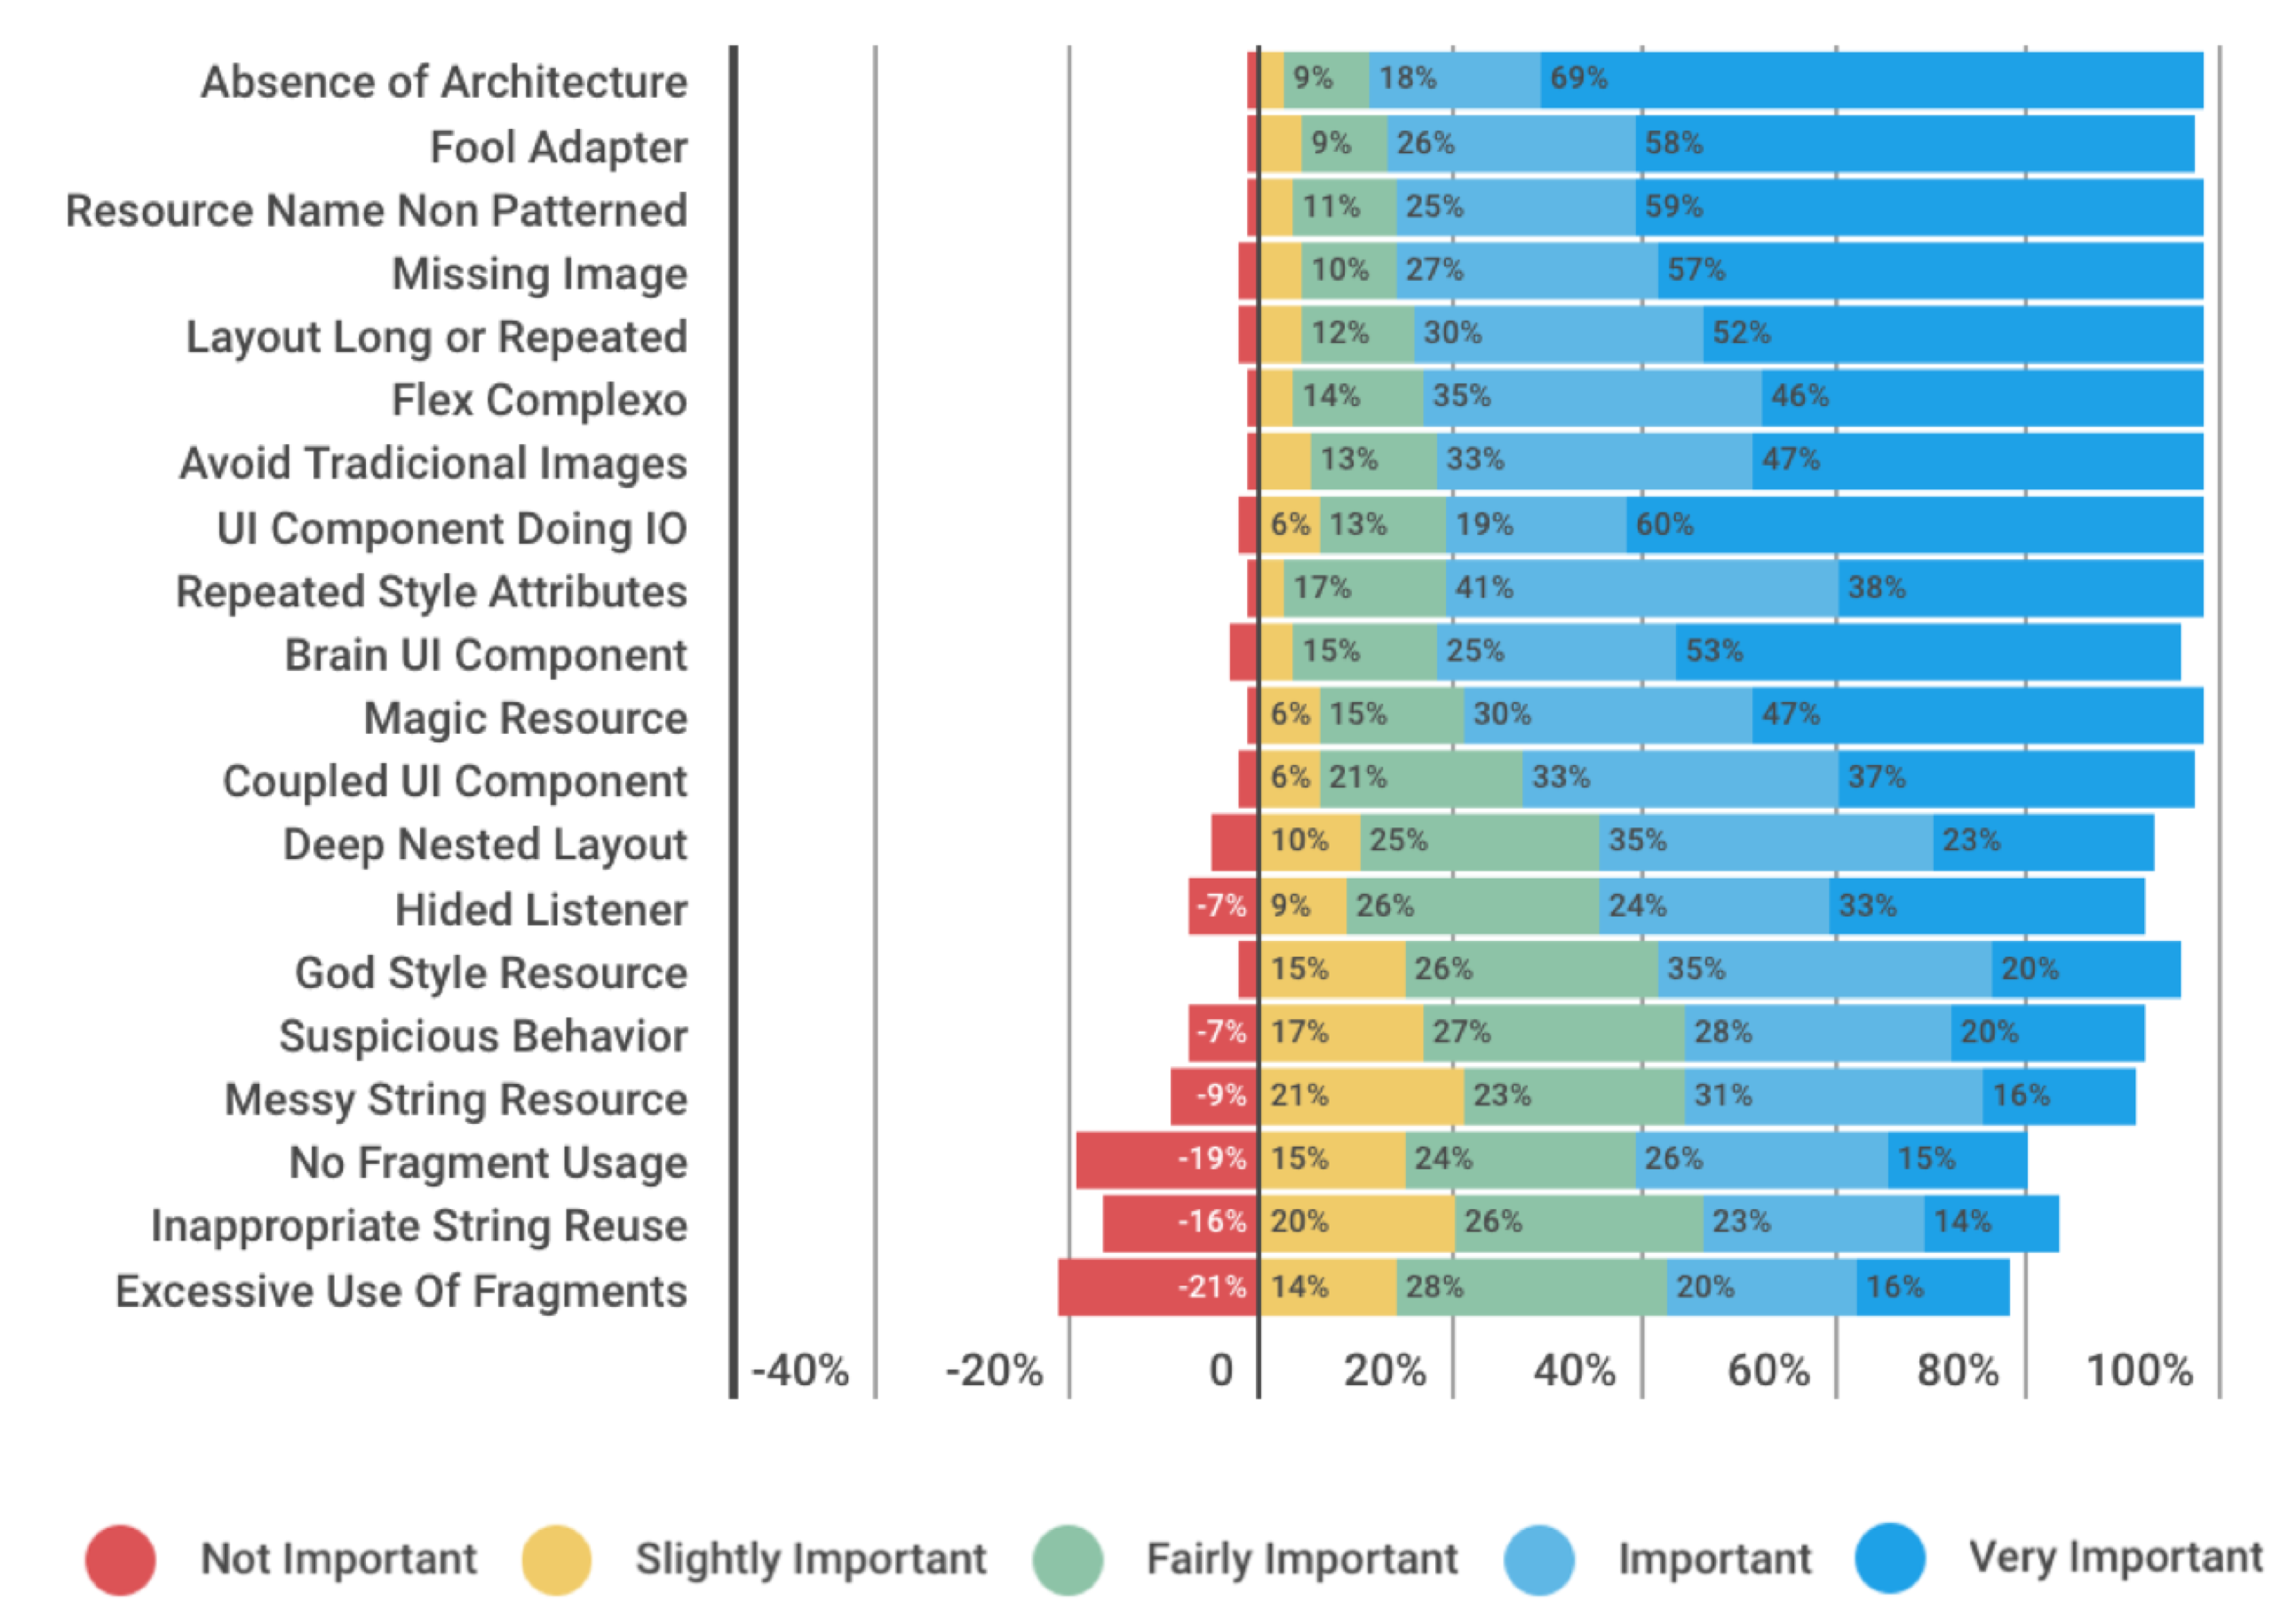
\includegraphics[width=1\textwidth]{phase2-results-importance3-en.png}
  \caption{Distribuição relativa de importância dos maus cheiros propostos.}
  \label{fig:phase2-results-importance}
  % \vspace{-.5cm}
\end{figure*}

Os três maus cheiros considerados menos importantes foram \textsc{\small Inappropriate String Reuse}, \textsc{\small No Fragment Usage} e \textsc{\small Uso Excessivo de Fragment}, com mais de 16\% dos participantes indicando ``não é importante'', menos de 26\% indicando ``importante'' e menos de 16\% indicando ``muito importante''. São os mesmos que tiveram menor concordância com relação à sua importância, todos com DP acima de 1,28. Esses dados sugerem que desenvolvedores Android ainda têm dúvidas sobre o impacto negativo desses maus cheiros no código.


\subsubsection{Frequência dos Maus Cheiros}

Para análise dos dados, simplificamos a escala \textit{likert} de frequência de modo similar ao de importância, onde maus cheiros de MO 2, ``raramente'', são classificados como \textbf{\small frequência baixa}, os maus cheiros de MO 3, ``às vezes'', são classificados como \textbf{\small frequência moderada} e os maus cheiros de MO 4 ou 5, respectivamente ``frequente'' e ``muito frequente'', são classificados de \textbf{\small frequência alta}. Nenhum mau cheiro teve MO 1, ``nunca'', e portanto não criamos classificação para essa opção. A Tabela \ref{tab:SmellFrequency} apresenta a lista dos maus cheiros de acordo com seu nível de frequência, alta, moderada ou baixa.

\begin{table}[!htb]
\centering
\renewcommand*{\arraystretch}{1}
\footnotesize
\caption{Listagem dos maus cheiros da camada de apresentação Android de acordo com seu nível de frequência, alta, moderada ou baixa.}
\begin{tabular}{@{}p{5.2cm}p{5.2cm}p{5.2cm}@{}}
\toprule
\multicolumn{1}{c}{\textbf{Frequência Alta}} & \multicolumn{1}{c}{\textbf{Frequência Moderada}} & \multicolumn{1}{c}{\textbf{Frequência Baixa}} \\
\bottomrule
\textsc{\scriptsize Repeated Style Attributes}  & \textsc{\scriptsize Flex Adapter}               & \textsc{\scriptsize Fool Adapter} \\
\textsc{\scriptsize Brain UI Component}       & \textsc{\scriptsize Absence of Architecture}        & \textsc{\scriptsize Hided Listener} \\
\textsc{\scriptsize Missing Image}                & \textsc{\scriptsize Classes de UI Fazendo IO}       & \textsc{\scriptsize No Fragment Usage} \\
\textsc{\scriptsize Avoid Tradicional Images} & \textsc{\scriptsize Coupled UI Component}      \\
\textsc{\scriptsize Layout Long or Repeated}       & \textsc{\scriptsize Uso Excessivo de Fragment}      \\
\textsc{\scriptsize Deep Nested Layout}  & \textsc{\scriptsize Suspicious Behavior}         \\
\textsc{\scriptsize God Style Resource}        & \textsc{\scriptsize Resource Name Non Patterned} \\
\textsc{\scriptsize Magic Resource}                 \\
\textsc{\scriptsize Inappropriate String Reuse}     \\
\textsc{\scriptsize Messy String Resource}    \\
\toprule
\multicolumn{1}{c}{10} & \multicolumn{1}{c}{7} & \multicolumn{1}{c}{3}\\
\bottomrule
\end{tabular}
\label{tab:SmellFrequency}
\end{table}

É interessante notar que, maus cheiros em recursos são percebidos mais frequentemente que os maus cheiros em componentes da camada de apresentação Android. Podemos observar na Tabela \ref{tab:SmellFrequency} que, 9 dentre os 10 maus cheiros de \textbf{\small frequência alta} são em recursos Android: \textsc{\small Repeated Style Attributes}, \textsc{\small Missing Image}, \textsc{\small Avoid Tradicional Images}, \textsc{\small Layout Long or Repeated}, \textsc{\small Deep Nested Layout}, \textsc{\small God Style Resource}, \textsc{\small Magic Resource}, \textsc{\small Inappropriate String Reuse} e \textsc{\small Messy String Resource}. Enquanto que apenas o mau cheiro de \textbf{\small frequência alta}, \textsc{\small Brain UI Component}, é relacionado a componentes da camada de apresentação Android.

Nos demais níveis de frequência, essa situação se inverte, sendo os maus cheiros em componentes da camada de apresentação Android, maioria. Dentre os maus cheiros de \textbf{\small frequência moderada}, 6 dentre os 7 são relacionados a componentes: \textsc{\small Flex Adapter}, \textsc{\small Absence of Architecture}, \textsc{\small Classes de UI Fazendo IO}, \textsc{\small Coupled UI Component}, \textsc{\small Uso Excessivo de Fragment} e \textsc{\small Suspicious Behavior}. Apenas o mau cheiro \textsc{\small Resource Name Non Patterned} é relacionado a recursos Android. Dentre os maus cheiro de \textbf{\small frequência baixa}, 2 dentre os 3 são relacionados a componentes da camada de apresentação Android: \textsc{\small Fool Adapter} e \textsc{\small No Fragment Usage}. E apenas o mau cheiro \textsc{\small Hided Listener} é relacionado a recursos Android.

\begin{figure*}[!htb]
  \centering
  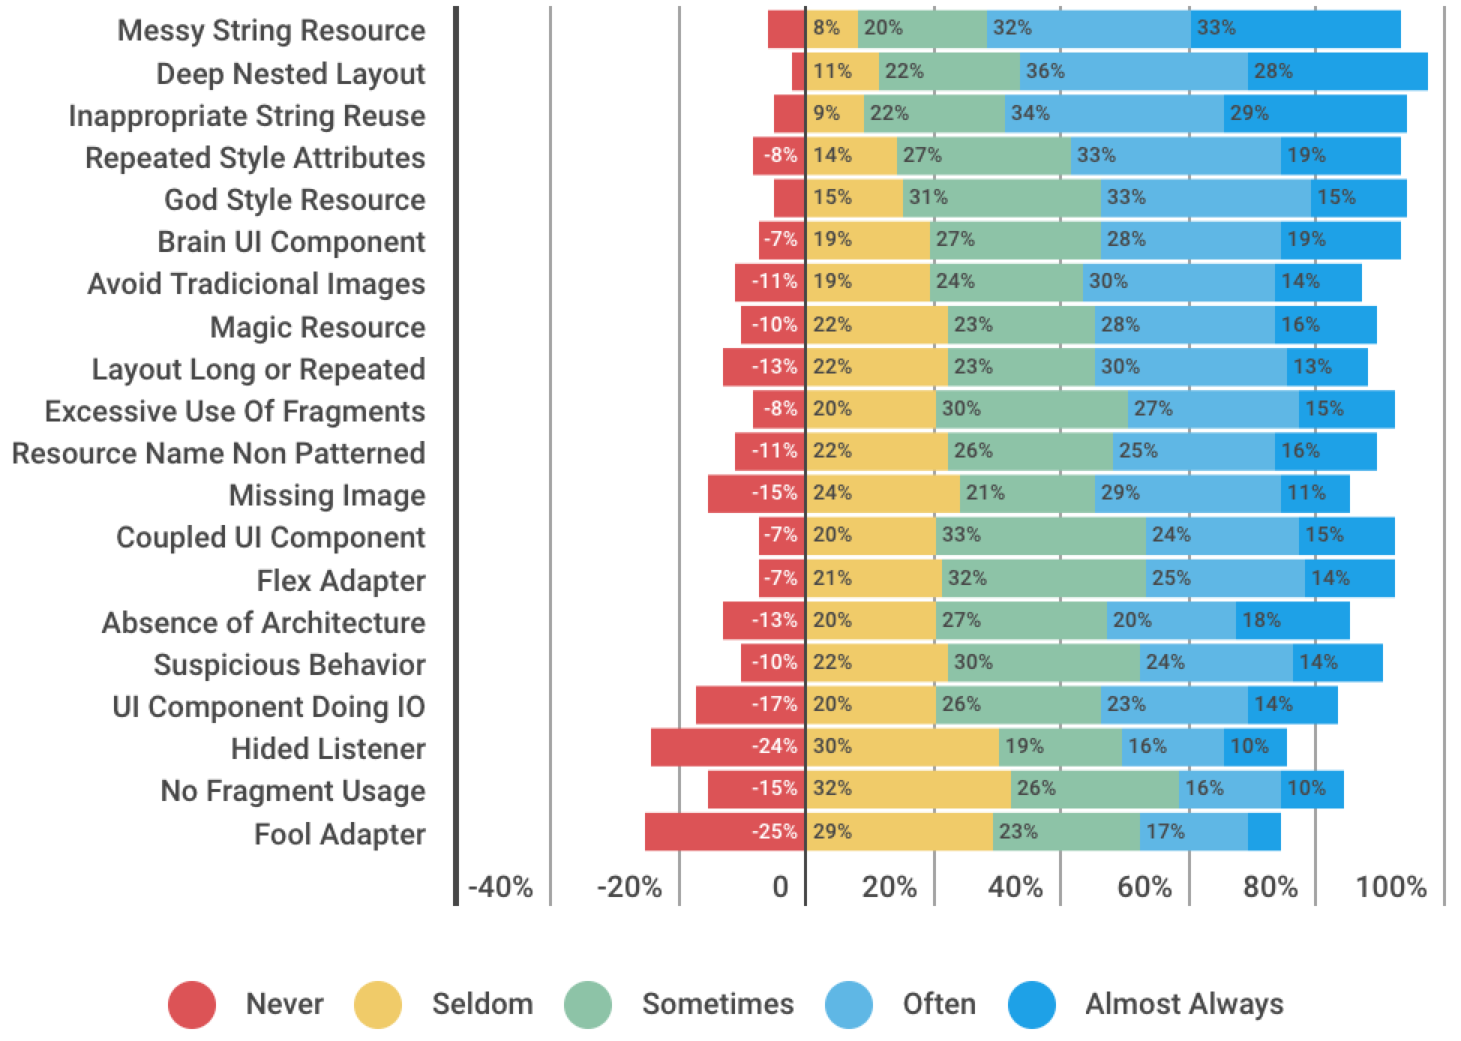
\includegraphics[width=1\textwidth]{phase2-results-frequence-en.png}
  \caption{Distribuição relativa de frequência dos maus cheiros propostos.}
  \label{fig:phase2-survey-frequence}
  % \vspace{-.5cm}
\end{figure*}

A Figura \ref{fig:phase2-survey-frequence} apresenta a distribuição relativa de frequência dos maus cheiros. Apresentamos negativo (em vermelho) o percentual relacionado às respostas ``nunca''. Os maus cheiros menos percebidos (com mais de 20\% de respostas ``nunca'') foram \textsc{\small Fool Adapter} (25\%) e \textsc{\small Hided Listener} (24\%). Todos os demais maus cheiros são percebidos no dia a dia, com frequência moderada ou alta, por pelo menos 75\% dos participantes.

\textsc{\small Fool Adapter} foi o mau cheiro menos percebido no dia a dia por desenvolvedores Android (25\% dos participantes indicaram ``nunca''). Entretanto ele é o segundo considerado mais importante (58\% dos participantes indicaram ``muito importante'' e 26\% indicaram ``importante''). Esses dados sugerem que desenvolvedores já estão cientes dos benefícios do uso do padrão \textit{ViewHolder} \cite{AluraViewHolder} e encontraram formas de mitigar este mau cheiro. Na seção \ref{sec:discussoes} realizamos uma breve discussão sobre esse resultado.

\textsc{\small Hided Listener} foi o segundo mau cheiro menos percebido no dia a dia por desenvolvedores Android (24\% dos participantes indicaram ``nunca''). Entretanto se apresenta dentre os maus cheiros considerados mais importantes (33\% dos participantes indicaram ``muito importante'' e 24\% indicaram ``importante''). Esses dados sugerem que os desenvolvedores consideram importante evitar o uso do atributo \textit{onClick} em XMLs de \textit{layout} e aparentemente, muitos desenvolvedores já estão cientes disso no dia a dia, uma vez que ele se apresenta dentre os 6 menos percebidos. \\


\begin{square}
  \small
  Nossos resultados mostram que os maus cheiros propostos são considerados importantes e frequentes no dia a dia do desenvolvimento Android (QP$_2$).
\end{square}




% -*- root: dissertation.tex -*-
\subsection{QP$_3$ Percepção dos Desenvolvedores sobre os Maus Cheiros Android}
\label{phase3-results}

Nossos resultados mostram que códigos afetados por 6 dos 7 maus cheiros avaliados são percebidos como códigos problemáticos por desenvolvedores Android, são eles: \textsc{\small Brain UI Component}, \textsc{\small Coupled UI Component}, \textsc{\small Suspicious Behavior}, \textsc{\small Flex Adapter}, \textsc{\small Deep Nested Layout} e \textsc{\small Repeated Style Attributes}. Não foi possível concluir a percepção sobre o mau cheiro \textsc{\small God Style Resource} pois a média de 30 pontos não foi suficiente para chegarmos a uma conclusão, sendo necessário coletar mais dados. A seguir apresentamos detalhes das percepções dos desenvolvedores sobre os maus cheiros avaliados.

% Com o objetivo de aumentar a confiabilidade do experimento, nosso objetivo foi obter em média 30 pontos de observação para cada mau cheiro avaliado. Para 6 maus cheiros essa quantidade de pontos foi suficiente, porém para o mau cheiro \textsc{\small God Style Resource} não,


\subsubsection{Resultados}
\label{sec:results-phase3}

Na Figura \ref{fig:components-violins}, apresentamos os gráficos violino que consolidam a percepção de desenvolvedores sobre os 4 maus cheiros relacionados a componentes da camada de apresentação Android (\textsc{\small Brain UI Component}, \textsc{\small Coupled UI Component}, \textsc{\small Suspicious Behavior} e \textsc{\small Flex Adapter}) contra componentes Android limpos. De modo similar, na Figura \ref{fig:resources-violins}, apresentamos os gráficos violino que consolidam a percepção de desenvolvedores sobre os 3 maus cheiros relacionados à recursos Android (\textsc{\small Deep Nested Layout}, \textsc{\small Repeated Style Attributes} e \textsc{\small God Style Resource}) contra recursos limpos.

\begin{figure*}[!htb]
\centering
\imagewidth=0.54\textwidth
\captionsetup[subfigure]{width=.9\imagewidth,justification=raggedright}%
\begin{subfigure}[t]{.49\textwidth}
  \centering
  \hspace*{-1cm}%
  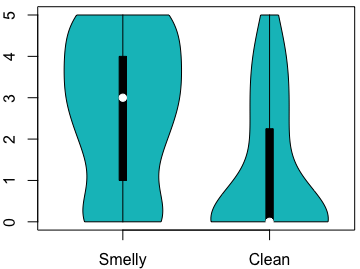
\includegraphics[width=.8\textwidth]{phase3-components-clean-smelly-violins-cutted-en.png}
  \caption{Components.}
  \label{fig:components-violins}
\end{subfigure}
\begin{subfigure}[t]{.49\textwidth}
  \centering
  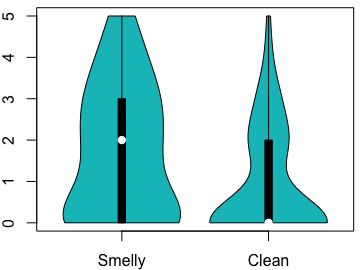
\includegraphics[width=.8\textwidth]{phase3-resources-clean-smelly-violins-cutted-en.png}
  \caption{Resources.}
  \label{fig:resources-violins}
\end{subfigure}%
\caption{Analysis of severity in components and resourcecs smelly and clean.}
\label{fig:smelly-clean-consolidado}
% \vspace{-.5cm}
\end{figure*}

No eixo y, 0 (zero) indica os códigos não percebidos pelos desenvolvedores como problemáticos (ou seja, responderam ``não'' à questão: ``\emph{Esta classe exibe algum problema de design e/ou implementação?}''), enquanto que os valores de 1 a 5 indicam o nível de severidade para o problema percebido pelo desenvolvedor. No eixo x, os gráficos são autoexplicativos. Nos parágrafos seguintes explicamos os dados de cada gráfico de modo que, as medianas são indicadas pela bolinha branca e o 3º quartil (Q3) é representado pela linha preta mais grossa na vertical.

Podemos observar na Figura \ref{fig:components-violins} que componentes afetados pelos maus cheiros Android tiveram mediana de severidade igual a 3 (Q3 = 4). Isso indica que, como esperado, desenvolvedores percebem códigos afetados pelos maus cheiros em componentes da camada de apresentação Android como problemáticos. Como comparação, componentes Android limpos tiveram mediana de severidade igual a 0 (Q3 = 2). A diferença na percepção dos desenvolvedores entre componentes Android mau cheirosos e componentes limpos é estatisticamente significante ($\alpha$ = 1,18e-06) com médio tamanho de efeito (\textit{d} = 0,46).

Na Figura \ref{fig:resources-violins}, podemos observar que recursos afetados pelos maus cheiros Android tiveram mediana de severidade é igual a 2 (Q3 = 3). Isso mostra que, recursos afetados pelos maus cheiros Android são percebidos como problemáticos, ainda que menos que os maus cheiros em componentes Android. Como comparação, recursos Android limpos tiveram mediana de severidade igual a 0 (Q3 = 2). A diferença na percepção dos desenvolvedores entre os recursos mau cheirosos e recursos limpos também é estatisticamente significante ($\alpha$ = 1,24e-03) com pequeno tamanho de efeito (\textit{d} = 0,29).

 % - bem como de componentes e recursos de \textit{Style} e \textit{Layout} limpos - Figura \ref{fig:clean-violins}.
Além disso, relatamos a percepção dos desenvolvedores sobre cada mau cheiro Android individualmente na Figura \ref{fig:smellys-violins}. O mau cheiro \textsc{\small Coupled UI Component} (CA) é o mais percebido pelos desenvolvedores e com maior gravidade, apresenta mediana de severidade igual a 4 (Q3 = 5). Em seguida temos os maus cheiros \textsc{\small Brain UI Component} (CC), \textsc{\small Flex Adapter} (AC) e \textsc{\small Suspicious Behavior} (CS) todos com mediana de severidade igual a 3. Isso indica que, como esperado, são percebidos pelos desenvolvedores como sendo seriamente problemáticos. Podemos notar que, de modo geral, recursos afetados pelos maus cheiros Android -- \textsc{\small God Style Resource} (LE), \textsc{\small Deep Nested Layout} (LA) e \textsc{\small Repeated Style Attributes} (AR) -- foram percebidos com menor severidade, mediana 1 e 2, do que componentes afetados pelos maus cheiros, todos com mediana de severidade maior ou igual a 3 (Q3 $\geq$ 3).  \\


\begin{figure*}[!htb]
\centering
\imagewidth=0.54\textwidth
\captionsetup[subfigure]{width=.9\imagewidth,justification=raggedright}%
\begin{subfigure}[t]{.48\textwidth}\centering
  \hspace*{-1cm}%
  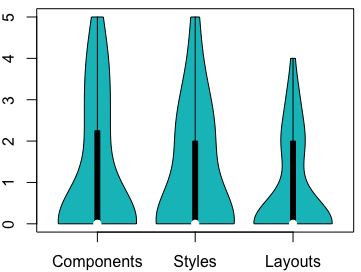
\includegraphics[width=.82\textwidth]{phase3-clean-violins-cutted-en.png}
  \caption{Components=\textit{Activities}, \textit{Fragments}, \textit{Adapters} or \textit{Listeners} cleans. Styles=Clean \textit{style} resources. Layout= Clean \textit{layout} resources.}
  % \hspace*{-1cm}%
  \label{fig:clean-violins}
\end{subfigure}
\begin{subfigure}[t]{.48\textwidth}\centering
  % \hspace*{-1cm}%
  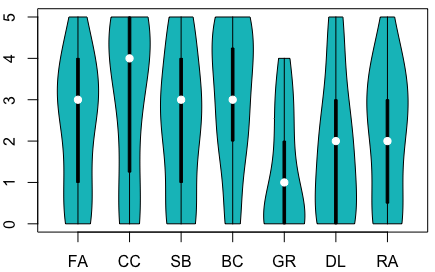
\includegraphics[width=1\textwidth]{phase3-smellys-violins2-cutted-en.png}
  \caption{FA=Flex Adapter, CC=Coupled UI Component, SB=Suspicious Behavior, BC=Brain UI Component, GR=God Style Resource, DL=Deep Nested Layout
, AR=Repeated Style Attributes.}
  % \hspace*{-1cm}%
  \label{fig:smellys-violins}
\end{subfigure}%
\caption{Analysis of severity of clean codes segmented by groups and codes affected by code smells evaluated.}
\label{fig:}
% \vspace{-.5cm}
\end{figure*}

A Figura \ref{fig:clean-violins} apresenta os gráficos violino sobre a percepção dos 3 grupos de códigos limpos: componentes Android, recursos de \textit{style} e recursos de \textit{layout}. Podemos observar que os 3 grupos de códigos apresentam mediana de severidade 0. Isso mostra que, como esperado, os códigos limpos, no geral, foram percebidos como limpos pelos desenvolvedores.

Muitos desenvolvedores, sem conhecer nosso catálogo de maus cheiros Android, foram capazes de identificar corretamente o mau cheiro, dando uma descrição do problema percebido muito próxima a definição do mau cheiro. Por exemplo, um deles ao se deparar com um \textsc{\small Flex Adapter} relatou: \textit{``O método getView é muito longo, com muitos ifs. Dificultando testes, debug e entendimento. me parece que muitas variações de tela podem ser desenhadas nesse método.''}. Outro participante disse simplesmente: \textit{``getView faz muitas coisas. Isso é perigoso para manter.''}.

Também o mau cheiro \textsc{\small God Style Resource}, foi corretamente identificado. Por exemplo, um dos participantes relatou: \textit{``Os temas e estilos poderiam ser separados em arquivos diferentes como por exemplo styles\_dialog.xml, styles\_text\_view.xml, etc inclusive em diretórios de recursos de acordo com nível de API do Android. Também poderia usar herança.''}. Outro participante disse apenas: \textit{``Muitos estilos no mesmo arquivo.''}.

Outro participante ao se deparar com \textsc{\small Coupled UI Component}, relatou: \textit{``Adapter está acoplado a MainActivity, uma vez que a recebe no construtor. O ideal seria abstrair quem está usando o Adapter para que ele possa ser usado por outras activities ou fragments.''}. Outros dois disseram simplesmente: \textit{``Cast direto à MainActivity.''} e \textit{``O DrawerAdapter está acoplado com a MainActivity.''}. Sobre o mau cheiro \textsc{\small Repeated Style Attributes}, um participante relatou: \textit{``1. Muitas dimensões repetidas que tem o mesmo propósito. Elas deveriam estar num lugar centralizado e nomeadas para facilidade de manutenção. 2. Mesma definição de estilo para várias text views. Deveria ser extraídas para styles para melhor manutenção...''}. Outro participante disse: \textit{``Muitos textViews com a mesma estilização, mas não se utiliza um arquivo de de styles para auxiliar.''}.

\begin{table}[!htb]
\centering
\renewcommand*{\arraystretch}{1}
\footnotesize
\caption{Dados estatísticos sobre a percepção negativa por desenvolvedores sobre os maus cheiros avaliados no experimento de código (S$_3$).}
\begin{tabular}{@{}p{7cm}clcc@{}}
\toprule
\textbf{Mau Cheiro} & \multicolumn{1}{c}{\textbf{Valor de p ($\alpha$)}} & \multicolumn{1}{c}{\textbf{Delta de Cliff (\textit{d})}} & \textbf{Mediana} & \textbf{Q3} \\
\toprule
\textsc{\small Coupled UI Component}       &  1,13e-04  &    0,52 (grande) & 4,00         & 5,00 \\
\textsc{\small Suspicious Behavior}          &  1,37e-03  &    0,38 (médio)  & 3,00         & 4,00 \\
\textsc{\small Brain UI Component}        &  4,58e-06  &    0,55 (grande) & 3,00         & 4,25 \\
\textsc{\small Flex Adapter}                &  1,11e-03  &    0,40 (médio)  & 3,00         & 4,00 \\
\textsc{\small God Style Resource}         &  7,61e-01  &    0,05 (insignificante) & 1,00 & 2,00 \\
\textsc{\small Deep Nested Layout}   &  6,17e-03  &    0,35 (médio)  & 2,00         & 3,00 \\
\textsc{\small Repeated Style Attributes}   &  5,84e-04  &    0,44 (médio)  & 2,00         & 3,00 \\
\bottomrule
\end{tabular}
\label{tab:smells-avaliados}
\end{table}


Foi possível confirmar estatisticamente a percepção dos desenvolvedores em 6 dos 7 maus cheiros Android avaliados. A Tabela \ref{tab:smells-avaliados} apresenta os valor de $\alpha$ e \textit{d} para todos eles, bem como informações de mediana e Q3. Apesar de haver respostas que identificaram corretamente o mau cheiro \textsc{\small God Style Resource} e do gráfico violino apresentar uma leve diferença de severidade dos recursos afetados pelo mau cheiro, com mediana 1 (Q3 = 2), contra os recursos limpos, são necessários mais dados para validá-lo estatisticamente. \\

\begin{square}
  \small
  Nossos resultados mostram que os códigos afetados pelos maus cheiros propostos e avaliados são percebidos como problemáticos por desenvolvedores Android se comparados com códigos limpos (QP$_3$).
\end{square}

